\chapter{Design and Methodology}
\label{ch:design}

This chapter presents the design of the system. The goals collected in Section~\ref{ch:design:goals} drive the structure, which is then described in three layers: data, simulation, and optimization. The relationship between the layers is captured in Figure~\ref{fig:design:architecture}, and the requirements are summarized in Table~\ref{tab:design:requirements}.

\begin{figure}[hbt!]
	\centering
	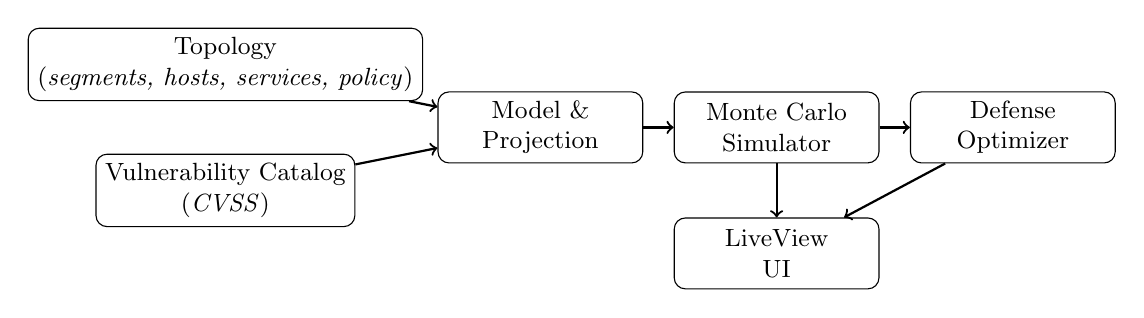
\begin{tikzpicture}[
			every node/.style={align=center, draw, rectangle, rounded corners, minimum width=2.6cm, minimum height=0.9cm, font=\small},
			arrow/.style={->, thick},
		]
		\node (topo)   at (0,  0)   {Topology\\(\textit{segments, hosts, services, policy})};
		\node (cve)    at (0,  -1.6) {Vulnerability Catalog\\(\textit{CVSS})};
		\node (graph)  at (4.0, -0.8) {Model \&\\Projection};
		\node (sim)    at (7.0, -0.8) {Monte Carlo\\Simulator};
		\node (opt)    at (10.0, -0.8) {Defense\\Optimizer};
		\node (ui)     at (7.0, -2.4) {LiveView\\UI};

		\draw[arrow] (topo)  -- (graph);
		\draw[arrow] (cve)   -- (graph);
		\draw[arrow] (graph) -- (sim);
		\draw[arrow] (sim)   -- (opt);
		\draw[arrow] (sim)   -- (ui);
		\draw[arrow] (opt)   -- (ui);
	\end{tikzpicture}
	\caption{Pipeline architecture: from data sources to optimizer and UI.}
	\label{fig:design:architecture}
\end{figure}

\section{Design Goals}
\label{ch:design:goals}

The system is designed to satisfy a small set of explicit goals. The goals are partitioned into functional and non-functional groups.

\begin{itemize}
	\item \textbf{Functional:}
	\begin{itemize}
		\item Construct a canonical graph with segment-policy reachability and derive operational flows for simulation.
		\item Simulate attacker propagation by Monte Carlo sampling and produce blast-radius and mission-impact outcomes.
		\item Recommend defensive actions (segment-policy removals, vulnerability patches) intended to reduce the modeled mission impact, with blast radius as a secondary safety outcome.
	\end{itemize}
	\item \textbf{Non-functional:}
	\begin{itemize}
		\item Reproducible results: a given topology and seed must produce the same blast-radius map across runs.
		\item Measurable scale: a benchmark over three controlled topology-size tiers must report median simulation, strategy-selection, and total-evaluation durations on a fixed documented environment after warm-up; no general scalability claim is made without such measurements.
		\item Implementation fits in a small number of Elixir source files, to make the system easy to study and modify~\cite{ou05mulval}.
	\end{itemize}
\end{itemize}

A compact view of the design is given in Table~\ref{tab:design:requirements}, which lists each requirement together with the section that elaborates on it.

\begin{table}[hbt!]
	\centering
	\begin{tabular}{lll}
		\toprule
		\textbf{ID} & \textbf{Requirement}            & \textbf{Elaboration} \\
		\midrule
		R1 & Topology ingest                 & Section~\ref{ch:design:data}       \\
		R2 & Vulnerability catalog           & Section~\ref{ch:design:data}       \\
		R3 & Context-graph construction      & Section~\ref{ch:design:graph}      \\
		R4 & Monte Carlo simulation          & Section~\ref{ch:design:sim}        \\
		R5 & Policy-based segmentation        & Section~\ref{ch:design:opt}        \\
		R6 & Greedy patch prioritization     & Section~\ref{ch:design:opt}        \\
		R7 & Annealing optimization            & Section~\ref{ch:design:opt}        \\
		R8 & LiveView-based UI               & Section~\ref{ch:design:ui}         \\
		\bottomrule
	\end{tabular}
	\caption{Design requirements and where each is elaborated in this chapter.}
	\label{tab:design:requirements}
\end{table}

\section{Data Layer}
\label{ch:design:data}

The data layer consists of two inputs. The first is a \emph{network topology}: a set of network segments, hosts, and services, together with a segment-to-segment reachability policy. Each policy rule permits the source segment to initiate traffic to matching services in the target segment and carries protocol and port-range data. The second is a \emph{vulnerability catalog} containing CVSS data and a separately assigned success probability. Generated topologies use a synthetic catalog. The fixed baseline may use a reviewed static NVD subset; a live NVD feed is not part of the implementation. CVSS describes severity characteristics, not a calibrated probability or real-world exploit likelihood~\cite{nvd}.

\section{Context-Graph Layer}
\label{ch:design:graph}

The graph layer stores the topology as a typed context graph. Hosts, services, and network segments are nodes; ownership (segment contains host, host runs service) and reachability are edges. Reachability is segment policy, not a host/service flow: the stored edge connects a source to a target segment and carries protocol and port-range data. The effective \enquote{host to service} flow is a deterministic projection materialized in memory when the simulator or the network view needs it. No flow is admitted unless a policy rule supports it, and no complete static attack graph is enumerated before simulation. The context graph and state-transition simulation are informed by attack-graph literature, including MulVAL~\cite{ou05mulval} and multiple-prerequisite graphs~\cite{ingols06mpg}; they are not an implementation of either attack-graph family.

\section{Simulation Layer}
\label{ch:design:sim}

The simulation layer runs a fixed number of Monte Carlo trials. Each trial starts at the configured entry point. At each state transition, the simulator evaluates eligible actions, selects one uniformly, then samples its outcome. Exploit actions use the vulnerability's independently assigned, stylized success probability; credential actions are deterministic when their preconditions hold. The probability is not derived from CVSS and is not calibrated to real-world exploitation. One trial reports its final set of compromised host footholds, including the initial foothold. The aggregate report gives their count distribution and the per-host empirical compromise probability.

\section{Optimization Layer}
\label{ch:design:opt}

The optimization layer takes simulated mission-impact and blast-radius outcomes with a budget $k$ of defensive actions. It returns actions selected under the configured objective. The thesis uses mission impact as the primary outcome and blast radius as a secondary safety outcome. Every current action has unit cost, so $k$ is an equal-action-count budget rather than a deployment-cost model. Simulation-informed and annealing strategies score candidates through simulation; CVSS-priority and topology-based strategies use direct rankings:

\begin{itemize}
	\item \textbf{Policy segmentation.} Remove a segment-policy rule. Each removal is a single canonical policy change, not a cut of individual host edges; the topology-based strategy ranks it by the reduction in deterministically reachable hosts after re-materializing the flows.
	\item \textbf{Simulation-informed patching.} Rank vulnerabilities by their marginal reduction under the selected simulation objective, measured by re-simulating each candidate graph, and patch the highest-ranked ones up to the budget.
	\item \textbf{Simulated annealing.} A stochastic search over patching and segmentation actions, guided by the selected simulated objective for each candidate graph.
\end{itemize}

\section{UI Layer}
\label{ch:design:ui}

The UI layer is a Phoenix LiveView application. It lets the user edit a graph, run simulations and optimizations, and inspect their reports. A simulation report can show a blast-radius heat map with mission-impact results.
